% Options for packages loaded elsewhere
\PassOptionsToPackage{unicode}{hyperref}
\PassOptionsToPackage{hyphens}{url}
%
\documentclass[
]{book}
\usepackage{amsmath,amssymb}
\usepackage{lmodern}
\usepackage{iftex}
\ifPDFTeX
  \usepackage[T1]{fontenc}
  \usepackage[utf8]{inputenc}
  \usepackage{textcomp} % provide euro and other symbols
\else % if luatex or xetex
  \usepackage{unicode-math}
  \defaultfontfeatures{Scale=MatchLowercase}
  \defaultfontfeatures[\rmfamily]{Ligatures=TeX,Scale=1}
\fi
% Use upquote if available, for straight quotes in verbatim environments
\IfFileExists{upquote.sty}{\usepackage{upquote}}{}
\IfFileExists{microtype.sty}{% use microtype if available
  \usepackage[]{microtype}
  \UseMicrotypeSet[protrusion]{basicmath} % disable protrusion for tt fonts
}{}
\makeatletter
\@ifundefined{KOMAClassName}{% if non-KOMA class
  \IfFileExists{parskip.sty}{%
    \usepackage{parskip}
  }{% else
    \setlength{\parindent}{0pt}
    \setlength{\parskip}{6pt plus 2pt minus 1pt}}
}{% if KOMA class
  \KOMAoptions{parskip=half}}
\makeatother
\usepackage{xcolor}
\IfFileExists{xurl.sty}{\usepackage{xurl}}{} % add URL line breaks if available
\IfFileExists{bookmark.sty}{\usepackage{bookmark}}{\usepackage{hyperref}}
\hypersetup{
  pdftitle={A primer for biostatistics in R},
  pdfauthor={cjlortie},
  hidelinks,
  pdfcreator={LaTeX via pandoc}}
\urlstyle{same} % disable monospaced font for URLs
\usepackage{color}
\usepackage{fancyvrb}
\newcommand{\VerbBar}{|}
\newcommand{\VERB}{\Verb[commandchars=\\\{\}]}
\DefineVerbatimEnvironment{Highlighting}{Verbatim}{commandchars=\\\{\}}
% Add ',fontsize=\small' for more characters per line
\usepackage{framed}
\definecolor{shadecolor}{RGB}{248,248,248}
\newenvironment{Shaded}{\begin{snugshade}}{\end{snugshade}}
\newcommand{\AlertTok}[1]{\textcolor[rgb]{0.94,0.16,0.16}{#1}}
\newcommand{\AnnotationTok}[1]{\textcolor[rgb]{0.56,0.35,0.01}{\textbf{\textit{#1}}}}
\newcommand{\AttributeTok}[1]{\textcolor[rgb]{0.77,0.63,0.00}{#1}}
\newcommand{\BaseNTok}[1]{\textcolor[rgb]{0.00,0.00,0.81}{#1}}
\newcommand{\BuiltInTok}[1]{#1}
\newcommand{\CharTok}[1]{\textcolor[rgb]{0.31,0.60,0.02}{#1}}
\newcommand{\CommentTok}[1]{\textcolor[rgb]{0.56,0.35,0.01}{\textit{#1}}}
\newcommand{\CommentVarTok}[1]{\textcolor[rgb]{0.56,0.35,0.01}{\textbf{\textit{#1}}}}
\newcommand{\ConstantTok}[1]{\textcolor[rgb]{0.00,0.00,0.00}{#1}}
\newcommand{\ControlFlowTok}[1]{\textcolor[rgb]{0.13,0.29,0.53}{\textbf{#1}}}
\newcommand{\DataTypeTok}[1]{\textcolor[rgb]{0.13,0.29,0.53}{#1}}
\newcommand{\DecValTok}[1]{\textcolor[rgb]{0.00,0.00,0.81}{#1}}
\newcommand{\DocumentationTok}[1]{\textcolor[rgb]{0.56,0.35,0.01}{\textbf{\textit{#1}}}}
\newcommand{\ErrorTok}[1]{\textcolor[rgb]{0.64,0.00,0.00}{\textbf{#1}}}
\newcommand{\ExtensionTok}[1]{#1}
\newcommand{\FloatTok}[1]{\textcolor[rgb]{0.00,0.00,0.81}{#1}}
\newcommand{\FunctionTok}[1]{\textcolor[rgb]{0.00,0.00,0.00}{#1}}
\newcommand{\ImportTok}[1]{#1}
\newcommand{\InformationTok}[1]{\textcolor[rgb]{0.56,0.35,0.01}{\textbf{\textit{#1}}}}
\newcommand{\KeywordTok}[1]{\textcolor[rgb]{0.13,0.29,0.53}{\textbf{#1}}}
\newcommand{\NormalTok}[1]{#1}
\newcommand{\OperatorTok}[1]{\textcolor[rgb]{0.81,0.36,0.00}{\textbf{#1}}}
\newcommand{\OtherTok}[1]{\textcolor[rgb]{0.56,0.35,0.01}{#1}}
\newcommand{\PreprocessorTok}[1]{\textcolor[rgb]{0.56,0.35,0.01}{\textit{#1}}}
\newcommand{\RegionMarkerTok}[1]{#1}
\newcommand{\SpecialCharTok}[1]{\textcolor[rgb]{0.00,0.00,0.00}{#1}}
\newcommand{\SpecialStringTok}[1]{\textcolor[rgb]{0.31,0.60,0.02}{#1}}
\newcommand{\StringTok}[1]{\textcolor[rgb]{0.31,0.60,0.02}{#1}}
\newcommand{\VariableTok}[1]{\textcolor[rgb]{0.00,0.00,0.00}{#1}}
\newcommand{\VerbatimStringTok}[1]{\textcolor[rgb]{0.31,0.60,0.02}{#1}}
\newcommand{\WarningTok}[1]{\textcolor[rgb]{0.56,0.35,0.01}{\textbf{\textit{#1}}}}
\usepackage{longtable,booktabs,array}
\usepackage{calc} % for calculating minipage widths
% Correct order of tables after \paragraph or \subparagraph
\usepackage{etoolbox}
\makeatletter
\patchcmd\longtable{\par}{\if@noskipsec\mbox{}\fi\par}{}{}
\makeatother
% Allow footnotes in longtable head/foot
\IfFileExists{footnotehyper.sty}{\usepackage{footnotehyper}}{\usepackage{footnote}}
\makesavenoteenv{longtable}
\usepackage{graphicx}
\makeatletter
\def\maxwidth{\ifdim\Gin@nat@width>\linewidth\linewidth\else\Gin@nat@width\fi}
\def\maxheight{\ifdim\Gin@nat@height>\textheight\textheight\else\Gin@nat@height\fi}
\makeatother
% Scale images if necessary, so that they will not overflow the page
% margins by default, and it is still possible to overwrite the defaults
% using explicit options in \includegraphics[width, height, ...]{}
\setkeys{Gin}{width=\maxwidth,height=\maxheight,keepaspectratio}
% Set default figure placement to htbp
\makeatletter
\def\fps@figure{htbp}
\makeatother
\setlength{\emergencystretch}{3em} % prevent overfull lines
\providecommand{\tightlist}{%
  \setlength{\itemsep}{0pt}\setlength{\parskip}{0pt}}
\setcounter{secnumdepth}{5}
\usepackage{booktabs}
\ifLuaTeX
  \usepackage{selnolig}  % disable illegal ligatures
\fi
\usepackage[]{natbib}
\bibliographystyle{apalike}

\title{A primer for biostatistics in R}
\author{cjlortie}
\date{}

\begin{document}
\maketitle

{
\setcounter{tocdepth}{1}
\tableofcontents
}
\hypertarget{introduction}{%
\chapter{Introduction}\label{introduction}}

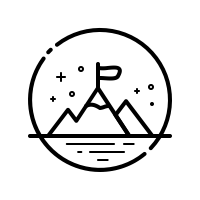
\includegraphics[width=4in,height=\textheight]{./adventure.png}

Welcome to a primer for biostatistics in R.

Mathematical! Adventure time! Well, the mathematical part is up to you, but this is an adventure. This set of learning materials is a guide developed to support you in better developing critical thinking using statistics. \href{https://www.criticalthinking.org/pages/defining-critical-thinking/766}{Critical thinking} very generally is a mode of thinking that is self-directed and evidence based \citep{RN6081}. Statistical thinking is thus an ideal opportunity and partner in honing literacy adventure skills in this domain. Enhancing clarity, accuracy, precision, relevance, depth, breadth, significance, logic and fairness - all key criteria of critical thinking - with data or evidence both quantitative and qualitative is a profound tool as a scientist and citizen. It should be fundamental to statistics. Hence, the primary goal of this set of materials is to engender statistical thinking that embodies these principles and explores these criteria using data.

The open and free resources associated with learning statistics is nearly infinite online particularly in R. The programming language \href{https://www.r-project.org}{R} is a free, open source programming environment ideal for statistics. There are other similar alternatives, but here R is used to support and scaffold critical thinking and statistical literacy because a significant component of many biologists \href{https://esajournals.onlinelibrary.wiley.com/doi/full/10.1002/ecs2.2567}{use R including ecologists} \citep{RN6098}. Importantly, it provides a simple and clear mechanism to document, annotate, tidy up, write down, and literally show your work - like in math class. This benefits you. You see your ideas written down and can explore logic, fairness, and all the criteria listed above. It also enables you to repeat, replicate, and share your work.

\hypertarget{course-outline}{%
\subsection*{Course outline}\label{course-outline}}
\addcontentsline{toc}{subsection}{Course outline}

If you are electing to engage with this learning opportunity formally, please see the official course outline for specific details.

There are two summative assessments.

\begin{enumerate}
\def\labelenumi{\arabic{enumi}.}
\tightlist
\item
  Write a \href{https://journals.plos.org/ploscompbiol/article?id=10.1371/journal.pcbi.1006562}{book review} for \href{https://global.oup.com/academic/product/the-new-statistics-with-r-9780198798187?cc=us\&lang=en\&}{The new Statistics with R.}\\
\item
  Complete a take-home statistical test (with the dataset provided in chapter 6 herein).
\end{enumerate}

\hypertarget{learning-outcomes}{%
\subsection*{Learning outcomes}\label{learning-outcomes}}
\addcontentsline{toc}{subsection}{Learning outcomes}

\begin{enumerate}
\def\labelenumi{\arabic{enumi}.}
\tightlist
\item
  Build a tidy, logical data model for a graduate-level dataset.\\
\item
  Develop a reproducible data and statistical workflow.\\
\item
  Design and complete intermediate-level data visualizations appropriate for a graduate-level tidy dataset.\\
\item
  Identify a range of suitable univariate or multivariate statistical approaches that can be applied to any dataset.\\
\item
  Interpret statistical output to quantify statistical model performance.\\
\item
  Complete fundamental exploratory data analysis on a representative dataset.\\
\item
  Appreciate the strengths and limitations of open science, data science, and evidence-based collaboration models.
\end{enumerate}

\hypertarget{steps}{%
\subsection*{Steps}\label{steps}}
\addcontentsline{toc}{subsection}{Steps}

Read a book. \href{https://global.oup.com/academic/product/the-new-statistics-with-r-9780198798187?cc=us\&lang=en\&}{The New Statistics with R.} \citep{RN7358}.

Write a book review. \href{https://journals.plos.org/ploscompbiol/article?id=10.1371/journal.pcbi.1006562}{Ten simple rules for writing statistical book reviews} \citep{RN6148} suggests a critical thinking framework to adopt for this process.

Learn-by-doing here.

Do a hackathon.

Do a hackathon as a test and submit for grading \& review.

\hypertarget{rationale}{%
\subsubsection*{Rationale}\label{rationale}}
\addcontentsline{toc}{subsubsection}{Rationale}

Some learn best by reading. Some learn best by doing. We can all benefit from both approaches to refining our critical thinking through statistics.

Two summative (i.e.~graded outcomes) include the book review and the test.

\hypertarget{schedule}{%
\subsection*{Schedule}\label{schedule}}
\addcontentsline{toc}{subsection}{Schedule}

Slide decks are optional. The decks simply highlight some of the connections between the criteria for critical thinking and statistical heuristics.

\begin{tabular}{rll}
\toprule
week & adventure & slide deck\\
\midrule
1 & {}[Tidy data in R](https://www.jstatsoft.org/article/view/v059i10) and CH9 in textbook & {}[whyR](https://figshare.com/articles/presentation/whyR\_why\_consider\_using\_R\_for\_your\_stats/15044448)\\
2 & {}[Literate statistical coding](https://ojs.library.queensu.ca/index.php/IEE/article/view/6559) and [Data science](https://www.jstatsoft.org/article/view/v077b01) and CH11 in texbook & {}[wrangleR](https://figshare.com/articles/presentation/wrangleR\_data\_wrangling\_in\_R/15044457)\\
3 & Statistics for ecology and evolution I and CH7 in textbook & {}[contemporary viz](https://figshare.com/articles/presentation/Contemporary\_data\_viz\_in\_R/15044445)\\
4 & Statistics for ecology and evolution II and CH15 in textbook & {}[EDAR](https://figshare.com/articles/presentation/Exploratory\_data\_analysis\_models\_in\_R/15044436)\\
5 & Book review due and hackathon & {}[efficient stats](https://figshare.com/articles/presentation/Efficient\_statistics/15044442)\\
\addlinespace
6 & Test & {}[when to publish data \& code](https://figshare.com/articles/presentation/The\_early\_bird\_gets\_the\_return\_when\_to\_publish\_your\_data/14681124)\\
\bottomrule
\end{tabular}

\hypertarget{instructions}{%
\subsection*{Instructions}\label{instructions}}
\addcontentsline{toc}{subsection}{Instructions}

Read the text at your own pace. At least hit the key chapters CH4, 10 \& 11 to write the review and submit your insights by the fifth week of work (if you choose to do 1-2 tasks per week as suggested in the schedule). If you are taking BIOL5081, please see official course outline and submit all work to \href{https://www.turnitin.com}{turnitin.com} as PDF only (even for the R work - knit to pdf).

Each week, read, discuss if you elect to work synchronously, and try the challenge provided.

The final two weeks, that hackathon is a warm up to the test. Grab the dataset, apply your critical thinking skills, code and show your work, and capture code and outputs as PDF. The hackathon is a stepping stone, formative process for to check if you are ready to think on your feet, write code, and apply biostatistical thinking to a challenge. The test is the exact same approach but summative, i.e.~you submit for review and grading to a peer or instructor like me.

\hypertarget{citation}{%
\subsection*{Citation}\label{citation}}
\addcontentsline{toc}{subsection}{Citation}

Lortie, CJ (2021): A primer for biostatistics in R. figshare. Book. \url{https://doi.org/10.6084/m9.figshare.15048597.v3}

\hypertarget{license}{%
\subsection*{License}\label{license}}
\addcontentsline{toc}{subsection}{License}

This work is licensed under a Creative Commons Attribution-NonCommercial-ShareAlike 4.0 International License.

\hypertarget{tidy-data-in-r}{%
\subsection*{Tidy data in R}\label{tidy-data-in-r}}
\addcontentsline{toc}{subsection}{Tidy data in R}

Tidiness is next to naturalness. We are wired up to see patterns and organize. Put that tendency to good work in data and statistical critical thinking.

\hypertarget{learning-outcomes-1}{%
\subsubsection*{Learning outcomes}\label{learning-outcomes-1}}
\addcontentsline{toc}{subsubsection}{Learning outcomes}

\begin{enumerate}
\def\labelenumi{\arabic{enumi}.}
\tightlist
\item
  Consider data structures such as long versus wide.\\
\item
  Read in a dataset to the R environment.\\
\item
  Do a t-test.
\end{enumerate}

\hypertarget{critical-thinking}{%
\subsubsection*{Critical thinking}\label{critical-thinking}}
\addcontentsline{toc}{subsubsection}{Critical thinking}

\href{https://www.jstatsoft.org/article/view/v059i10}{Tidy data} thinking was pioneered in the R world \citep{RN4416}. This philosophy to first considering the basic format of your data is transformational and profound. It beautifully connects to logic. Better yet, it sets you up for easier stats and plots in many environments including R. There is an excellent \href{https://r4ds.had.co.nz/tidy-data.html}{chapter} on this topic in the free, open text R for Data Science.

\hypertarget{adventure-time}{%
\subsubsection*{Adventure time}\label{adventure-time}}
\addcontentsline{toc}{subsubsection}{Adventure time}

Very simple life data to explore some ideas about meditation, steps, resting heart rate and the importance of instrument variation. Data are \href{https://figshare.com/articles/dataset/Simple_health_data/15040515}{here}. Explore the t-test in R for this adventure. Is the number of steps or sleep different from 0? Do the means estimated from a watch versus simple Fitbit tracker vary for simple measures? Did 0 versus 12 mins of meditation per day influence a relevant measure?

Deeper dive: explore the var.equal or alternative argument. Test nonparametric analog to this test.

\begin{Shaded}
\begin{Highlighting}[]
\FunctionTok{library}\NormalTok{(tidyverse)}
\NormalTok{simple\_life }\OtherTok{\textless{}{-}} \FunctionTok{read\_csv}\NormalTok{(}\FunctionTok{url}\NormalTok{(}\StringTok{"https://ndownloader.figshare.com/files/28920855"}\NormalTok{))}
\NormalTok{simple\_life}
\end{Highlighting}
\end{Shaded}

\begin{verbatim}
## # A tibble: 9 x 7
##   simple_date steps_fitbit sleep_fitbit    hr steps_watch sleep_watch
##   <date>             <dbl>        <dbl> <dbl>       <dbl>       <dbl>
## 1 2021-06-02         20913          429    54       25197         314
## 2 2021-06-03          6904          447    53       13042         302
## 3 2021-06-04         19548          449    56       23285         413
## 4 2021-06-05         19311          423    56       25832         355
## 5 2021-06-06         26159          435    58       29533         385
## 6 2021-06-07         21618          358    56       27796         240
## 7 2021-06-08         20890          492    53       24360         434
## 8 2021-06-09         12008          541    53       14517         399
## 9 2021-06-10         18058          436    57       22392         403
## # ... with 1 more variable: meditation_mins <dbl>
\end{verbatim}

\hypertarget{reflection-questions}{%
\subsubsection*{Reflection questions}\label{reflection-questions}}
\addcontentsline{toc}{subsubsection}{Reflection questions}

\begin{enumerate}
\def\labelenumi{\arabic{enumi}.}
\tightlist
\item
  What can a t-test do? Can you imagine other functions for a t-test in the context of your work and life?
\item
  What are the limitations of a t-test?
\item
  Is the data structure wide, long, and how can you consider tidying this evidence? Are there variables that represent the same concept?
\end{enumerate}

\hypertarget{coding}{%
\chapter{Literate coding}\label{coding}}

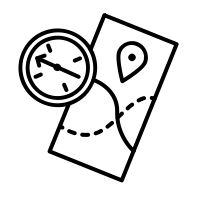
\includegraphics[width=3in,height=\textheight]{./coding.png}

Your code is a story too. Use your code and annotation of decisions (en)coded in your data manipulations, calculations, models, and plots to communicate clarity, logic, relevance, and depth. This story is not just for your collaborators - it is for you. Writing down your ideas and work down makes it more clear. It also reminds you later, even a week later, why you elected to make a particular decision in your workflow. Tidy data and tidy thinking make for better science.

\hypertarget{learning-outcomes-2}{%
\subsubsection*{Learning outcomes}\label{learning-outcomes-2}}
\addcontentsline{toc}{subsubsection}{Learning outcomes}

\begin{enumerate}
\def\labelenumi{\arabic{enumi}.}
\tightlist
\item
  Practice writing code and using annotation.\\
\item
  Consolidate your understanding of tidy data and critical thinking statistically.\\
\item
  Do an ANOVA.
\end{enumerate}

\hypertarget{critical-thinking-1}{%
\subsubsection*{Critical thinking}\label{critical-thinking-1}}
\addcontentsline{toc}{subsubsection}{Critical thinking}

Tidy data make your life easier. Data structures should match intuition and common sense. Data should have logical structure. Rows are are observations, columns are variables. Tidy data also increase the viability that others can use your data, do better science, reuse science, and help you and your ideas survive and thrive.

Literate coding \citep{RN4414} should capture a workflow that includes the wrangling you did to get your data ready. Literate code should be able to read by a human AND a machine. If data are already very clean in a spreadsheet, they can easily become a literate, logical dataframe. Nonetheless, you should still use annotation within the introductory code to explain the meta-data of your data to some extent and what you did pre-R to get it tidy. The philosophy here is very similar to the data viz lesson forthcoming that promotes critical thinking statistically through documented and described steps that are replicable and clear.

\hypertarget{adventure-time-1}{%
\subsubsection*{Adventure time}\label{adventure-time-1}}
\addcontentsline{toc}{subsubsection}{Adventure time}

Many years ago in a galaxy far, far away, a student sowed seeds in the desert at different densities for their PhD research. Here are the \href{https://figshare.com/articles/dataset/Density_experiment_in_Negev_Desert_Israel/669703}{data}, and here is the \href{https://besjournals.onlinelibrary.wiley.com/doi/10.1046/j.1365-2745.2002.00686.x}{publication} too \citep{RN3094}. This student was not strong in the force, but it was a good adventure in beginning to understand the relative importance of significance biologically and statistically by exploring critical thinking. For your adventure, test whether a set of groups differ from one another. For instance, test whether transects, or years, or even the density of seeds planted differs in an outcome measure such as mean plant size.

Deeper dive: Check for homoscedasticity or do a post-hoc test.

\begin{Shaded}
\begin{Highlighting}[]
\FunctionTok{library}\NormalTok{(tidyverse)}
\NormalTok{density }\OtherTok{\textless{}{-}} \FunctionTok{read\_csv}\NormalTok{(}\FunctionTok{url}\NormalTok{(}\StringTok{"https://ndownloader.figshare.com/files/28934310"}\NormalTok{))}
\NormalTok{density}
\end{Highlighting}
\end{Shaded}

\begin{verbatim}
## # A tibble: 152 x 6
##     year transect seed_density_pe~ final_plant_den~ survivorship mean_plant_size
##    <dbl>    <dbl>            <dbl>            <dbl>        <dbl>           <dbl>
##  1  1998        1           0.0625               41        0.461           0.554
##  2  1998        1           0.0625               47        0.712           0.356
##  3  1998        1           0.0625               60        0.698           0.301
##  4  1998        1           0.25                 31        0.525           0.808
##  5  1998        1           0.25                 50        0.505           0.212
##  6  1998        1           0.25                 58        0.563           0.148
##  7  1998        1           1                    30        0.273           0.578
##  8  1998        1           1                    42        0.243           1.28 
##  9  1998        1           1                    73        0.619           0.719
## 10  1998        1           2                    46        0.263           0.652
## # ... with 142 more rows
\end{verbatim}

\hypertarget{reflection-questions-1}{%
\subsubsection*{Reflection questions}\label{reflection-questions-1}}
\addcontentsline{toc}{subsubsection}{Reflection questions}

\begin{enumerate}
\def\labelenumi{\arabic{enumi}.}
\tightlist
\item
  What is the difference between a t-test and an ANOVA?\\
\item
  What is the difference between an ANOVA and GLM?\\
\item
  What are some of the ways that these simple data can be further analyzed?\\
\item
  When you explored annotation and describing your decisions and workflow for these data adventure, was it logical and clear to you if you ignored the R code?
\end{enumerate}

\hypertarget{eebI}{%
\chapter{Stats used in eeb I}\label{eebI}}


\includegraphics[width=3in,height=\textheight]{./eebI.png}

Many approaches and critical thinking heuristics in ecology \& evolutionary biology (eeb) are relevant to other disciplines.

\hypertarget{learning-outcomes-3}{%
\subsubsection*{Learning outcomes}\label{learning-outcomes-3}}
\addcontentsline{toc}{subsubsection}{Learning outcomes}

\begin{enumerate}
\def\labelenumi{\arabic{enumi}.}
\tightlist
\item
  Develop your data viz skills.\\
\item
  Hone your critical thinking statistically by iterative plotting-modeling a dataset.\\
\item
  Do a regression analysis.
\end{enumerate}

\hypertarget{critical-thinking-2}{%
\subsubsection*{Critical thinking}\label{critical-thinking-2}}
\addcontentsline{toc}{subsubsection}{Critical thinking}

Clean simple graphics are powerful tools in statistics (and in scientific communication). \href{https://www.edwardtufte.com/tufte/}{Tufte} \citep{RN2096} and others have shaped data scientists and statisticians in developing more libraries, new standards, and assumptions associated with graphical representations of data. Data viz must highlight the differences, show underlying data structures, and provide insights into the specific research project. R is infinitely customizable in all these respects. There are at least two major current paradigms (there are more these are the two dominant idea sets). Base R plots are simple, relatively flexible, and very easy. However, their grammar, i.e their rules of coding are not modern. Ggplot and related libraries invoke a new, formal grammar of graphics \citep{RN7256} that is more logical, more flexible, but divergent from base R code. It is worth the time to understand the differences and know when to use each.

Evolution of plotting in statistics using R in particular went from base-R then onto lattice then to the ggvis universe with the most recent library being ggplot \citep{RN4413}. Base-R is certainly useful in some contexts as is the lattice and lattice extra library. However, ggplot now encompasses all these capacities with a much simpler set of grammar (i.e.~rules and order). Nonetheless, you should be able to read base-R code for plots and be able to do some as well. The philosophy or grammar of modern graphics is well articulated and includes the following key principles. The grammar of graphics layers primacy of ideas (simple first, then more complex) i.e.~you build up your plots data are mapped to aesthetic attributes and geometric objects data first then statistics even in plots \citep{RN7255}. This directly supports critical thinking statistically because it promotes depth (literally), precision, and also accuracy in the decisions you make to show your evidence.

\hypertarget{adventure-time-2}{%
\subsubsection*{Adventure time}\label{adventure-time-2}}
\addcontentsline{toc}{subsubsection}{Adventure time}

Here are a deeper set of quantified life \href{https://figshare.com/articles/dataset/Quantified_life/12803105}{data}. Explore whether movement predicts total sleep or its efficiency. Plot out some patterns first, then, do a regression.

Deeper dive: explore residuals and try the cooks.distance function for outliers.

\begin{Shaded}
\begin{Highlighting}[]
\FunctionTok{library}\NormalTok{(tidyverse)}
\NormalTok{life }\OtherTok{\textless{}{-}} \FunctionTok{read\_csv}\NormalTok{(}\FunctionTok{url}\NormalTok{(}\StringTok{"https://ndownloader.figshare.com/files/28920729"}\NormalTok{))}
\NormalTok{life}
\end{Highlighting}
\end{Shaded}

\begin{verbatim}
## # A tibble: 4,561 x 7
##    simple_date  year steps mins_asleep efficiency lagged_sleep lagged_efficiency
##    <date>      <dbl> <dbl>       <dbl>      <dbl>        <dbl>             <dbl>
##  1 2011-01-25   2011 13900         481         96          504                99
##  2 2011-01-26   2011 19229         478         96          481                96
##  3 2011-01-27   2011 13103         474         96          478                96
##  4 2011-01-28   2011  7374         491         96          474                96
##  5 2011-01-29   2011 19132         436         96          491                96
##  6 2011-01-30   2011 17157         447         98          436                96
##  7 2011-01-31   2011 19759         456         99          447                98
##  8 2011-02-01   2011 18157         455         98          456                99
##  9 2011-02-02   2011  8768         465         97          455                98
## 10 2011-02-03   2011  9150         411         98          465                97
## # ... with 4,551 more rows
\end{verbatim}

\hypertarget{reflection-questions-2}{%
\subsubsection*{Reflection questions}\label{reflection-questions-2}}
\addcontentsline{toc}{subsubsection}{Reflection questions}

\begin{enumerate}
\def\labelenumi{\arabic{enumi}.}
\tightlist
\item
  When do you use regression versus correlation?\\
\item
  How could you incorporate time into your plots or statistical models?\\
\item
  Did the visualization highlight some of the criteria associated with critical thinking statistically more than others?
\end{enumerate}

\hypertarget{eebII}{%
\chapter{Stats used in eeb II}\label{eebII}}

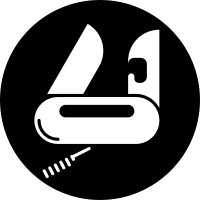
\includegraphics[width=3in,height=\textheight]{./eebII.png}

There is much counting in ecology \& evolutionary biology (eeb) \citep{RN7219}. We count individuals, species, populations, interactions, and then map out diversity and distributions to infer process. Many disciplines use similar logic in the structure of their evidence and experimental design with statistics.

\hypertarget{learning-outcomes-4}{%
\subsubsection*{Learning outcomes}\label{learning-outcomes-4}}
\addcontentsline{toc}{subsubsection}{Learning outcomes}

\begin{enumerate}
\def\labelenumi{\arabic{enumi}.}
\tightlist
\item
  Practice your critical workflow for data and statistics that is replicable and literate.\\
\item
  Appreciate the value of generalized statistical models that connect to one another conceptually.\\
\item
  Do a GLM.
\end{enumerate}

\hypertarget{critical-thinking-3}{%
\subsubsection*{Critical thinking}\label{critical-thinking-3}}
\addcontentsline{toc}{subsubsection}{Critical thinking}

Exploratory data analyses is everything we have done. This is a primary approach to better understanding your evidence without introducing bias. Transparency is key.

Workflow we have developed but that you nuance based on your cognitive and critical thinking style and strengths.

\begin{enumerate}
\def\labelenumi{\alph{enumi}.}
\tightlist
\item
  Tidy data.\\
\item
  Inspect data structure.\\
\item
  Data viz.\\
\item
  Basic exploratory data analyses.
\end{enumerate}

However, now that we are ready to apply models, we add in one more tiny step. Continue to visualize the data to better understand its typology and underlying distribution. Then, you are ready to fit your models. Exploratory data analyses is an intermediate step to this end. EDA includes testing assumptions in the data, fitting basic models that ignore covariates, fitting relevant and logical models to explore the data, training your data, and exploring sensitivity \citep{RN1755}. This process builds a viable path for further inquiry, and it is a model builder that is predicated upon critital thinking to ensure you inference (deduction, induction) is aligned with your evidence \citep{RN6096}.

A statistical model is an elegant, representative simplification of the patterns you have identified through data viz and EDA \citep{RN6911}. It is a formal mathematical relationship between factors of interest. It should capture data/experimental structure including the key variables, appropriate levels, and relevant covariation or contexts that mediate outcomes. It should support the data viz.~It should provide an estimate of the statistical likelihood or probability of differences. Ideally, the underlying coefficients should also be mined to convey an estimate of effect sizes. A t.test, chi.square test, regression/linear model, general linear model, or generalized linear mixed model are all examples of models that describe and summarize patterns and each have associated assumptions about the data they embody. Hence, the final step pre-model fit, is explore distributions.

Conceptually, there are two kind of models. Those that look back and those that look forward. Think tardis or time machine. A model is always a snapshot using your time machine. It can be a grab of what happened or a future snap of what you predict. In R, there is simple code to time travel in either direction. Actually, there is no time - Arrow of time - only an observer potential perception of it. Statistical models are our observers here. These observers use `probability distributions' as we described in the first week sensu statistical thinking to calibrate what the think critically when observed or will observe given the evidence at hand. Here are two super resources to further support this in a proximate sense that align with critical thinking. \href{https://med.cmb.ac.lk/SMJ/VOLUME\%203\%20DOWNLOADS/Page\%2033-37\%20-\%20Choosing\%20the\%20correct\%20statistical\%20test\%20made\%20easy.pdf}{Choosing the correct statistical test made easy} \citep{RN7257}, and a \href{./flowchart.jpg}{flowchart} for selecting commonly used statistics developed by Bates College.

\hypertarget{adventure-time-3}{%
\subsubsection*{Adventure time}\label{adventure-time-3}}
\addcontentsline{toc}{subsubsection}{Adventure time}

Here is an impressive \href{https://knb.ecoinformatics.org/view/doi\%3A10.5063\%2F6M357V}{dataset} describing bird counts in Toronto. These data were collected by York University undergraduates in an experimental design course. Explore whether there is a bias in detection by behaviour and identify the most common species by location in Toronto - at least as estimated using these data. For your curiosity, here are data collected in another larger citizen science endeavour - The \href{https://knb.ecoinformatics.org/view/doi\%3A10.5063\%2FF1RF5SDJ}{Christmas Bird Count for Southern Ontario region centered around the Greater Toronto Area}.

Deeper dive: If you wish to adventure further afield, contrast the two datasets. Explore fitting a different family to the data or explore offset argument versus covariates.

\begin{Shaded}
\begin{Highlighting}[]
\FunctionTok{library}\NormalTok{(tidyverse)}
\NormalTok{birds }\OtherTok{\textless{}{-}} \FunctionTok{read\_csv}\NormalTok{(}\FunctionTok{url}\NormalTok{(}\StringTok{"https://knb.ecoinformatics.org/knb/d1/mn/v2/object/urn\%3Auuid\%3Aa84a9673{-}878a{-}4c43{-}ba08{-}570b2d38bdc9"}\NormalTok{))}
\NormalTok{birds}
\end{Highlighting}
\end{Shaded}

\begin{verbatim}
## # A tibble: 826 x 11
##     year experiment      source   rep date  location species frequency behaviour
##    <dbl> <chr>           <chr>  <dbl> <chr> <chr>    <chr>       <dbl> <chr>    
##  1  2020 balcony birdwa~ full       1 10/1~ Holditc~ Agelai~         3 flying   
##  2  2020 balcony birdwa~ full       1 10/1~ Holditc~ Agelai~         4 flying   
##  3  2020 balcony birdwa~ full       1 10/1~ Holditc~ Agelai~         1 perching 
##  4  2020 balcony birdwa~ full       1 10/1~ High Pa~ Aix sp~         4 swimming 
##  5  2020 balcony birdwa~ full       1 10/9~ Vaughan  Anas p~         4 flying   
##  6  2020 balcony birdwa~ full       1 10/9~ Vaughan  Anas p~         6 flying   
##  7  2020 balcony birdwa~ full       1 10/9~ Vaughan  Anas p~         9 flying   
##  8  2020 balcony birdwa~ full       1 10/9~ Vaughan  Anas p~        10 flying   
##  9  2020 balcony birdwa~ full       1 10/9~ Vaughan  Anas p~         2 inactive 
## 10  2020 balcony birdwa~ full       1 10/9~ Vaughan  Anas p~         2 inactive 
## # ... with 816 more rows, and 2 more variables: inititals <chr>,
## #   citation_DOI <chr>
\end{verbatim}

\hypertarget{reflection-questions-3}{%
\subsubsection*{Reflection questions}\label{reflection-questions-3}}
\addcontentsline{toc}{subsubsection}{Reflection questions}

\begin{enumerate}
\def\labelenumi{\arabic{enumi}.}
\tightlist
\item
  When do you move from EDA to model fitting?\\
\item
  Are there ways to mitigate bias and \href{https://www.wired.com/story/were-all-p-hacking-now/}{p-hacking} through formal workflows?\\
\item
  Did building a model such as GLM align with critical thinking and intuition, i.e from critical thinking was it accurate and fair? Did the EDA-to-model process legitimately represent the patterns in the observations recorded.
\end{enumerate}

\hypertarget{hackathon}{%
\chapter{Hackathon}\label{hackathon}}


\includegraphics[width=3in,height=\textheight]{./hackathon.png}

All models are wrong but some are useful \citep{RN6467, RN7258}. Critical thinking with statistics is thus critical to ensure that we effectively support evidence informed decision making in society \citep{RN6861, RN7180}.

\hypertarget{learning-outcomes-5}{%
\subsubsection*{Learning outcomes}\label{learning-outcomes-5}}
\addcontentsline{toc}{subsubsection}{Learning outcomes}

\begin{enumerate}
\def\labelenumi{\arabic{enumi}.}
\tightlist
\item
  Appreciate the challenge of working with data to apply a critical thinking \& creative design mindset to statistical solutions.\\
\item
  Practice your workflow and literate coding before a summative test.\\
\item
  Refine your thinking and coding for efficiency.
\end{enumerate}

\hypertarget{critical-thinking-4}{%
\subsubsection*{Critical thinking}\label{critical-thinking-4}}
\addcontentsline{toc}{subsubsection}{Critical thinking}

\href{https://en.wikipedia.org/wiki/Efficiency_(statistics)}{Efficiency} is a fascinating topic in statistics \citep{RN7261, RN7260, RN7259}. Here, we can simplify this using the critical thinking criteria we have extensively refined and applied to numerous, tidy challenges. Efficiency = sufficiency (provided it is logical, fair, and accurate). Your plots and statistical models should represent a reasonable and likely description of the data at hand. This section is a formative opportunity for you to evaluate your skills and strengths in logic, efficiency, fair adventuring, workflows, and literate coding prior to the final section - a test. You are provided with a general dataset(s). The adventure is solve a very generalized challenge that is embodied in the evidence.

\hypertarget{adventure-time-4}{%
\subsubsection*{Adventure time}\label{adventure-time-4}}
\addcontentsline{toc}{subsubsection}{Adventure time}

Candy. Candy. Candy. Take a peek at these sweet data. Contrast Canada and USA candy sales at Halloween. Considering including population density in your model for each country for each year so as not to introduce variation and to be more accurate in estimating meaningful differences.

\href{https://figshare.com/articles/dataset/Canadian_Candy_Sales/9876386}{Canadian Candy}\\
\href{https://figshare.com/articles/dataset/USA_Halloween_spending/13125572}{USA Candy \& Halloween spending}\\
\href{https://figshare.com/articles/dataset/World_human_populations/16746652}{Human populations}

Deeper dive: contrast GLMM model performance, examine temporal effects, or explore GAMs.

\begin{Shaded}
\begin{Highlighting}[]
\FunctionTok{library}\NormalTok{(tidyverse)}
\NormalTok{Canada }\OtherTok{\textless{}{-}} \FunctionTok{read\_csv}\NormalTok{(}\FunctionTok{url}\NormalTok{(}\StringTok{"https://figshare.com/ndownloader/files/30990820"}\NormalTok{))}
\NormalTok{Canada}
\end{Highlighting}
\end{Shaded}

\begin{verbatim}
## # A tibble: 233 x 3
##    month  year  candy
##    <dbl> <dbl>  <dbl>
##  1     1  1997 101014
##  2     2  1997 101938
##  3     3  1997 136057
##  4     4  1997 105601
##  5     5  1997 119123
##  6     6  1997 107689
##  7     7  1997 113399
##  8     8  1997 113934
##  9     9  1997 109441
## 10    10  1997 146876
## # ... with 223 more rows
\end{verbatim}

\begin{Shaded}
\begin{Highlighting}[]
\NormalTok{USA }\OtherTok{\textless{}{-}} \FunctionTok{read\_csv}\NormalTok{(}\FunctionTok{url}\NormalTok{(}\StringTok{"https://figshare.com/ndownloader/files/25190510"}\NormalTok{))}
\NormalTok{USA}
\end{Highlighting}
\end{Shaded}

\begin{verbatim}
## # A tibble: 16 x 6
##     year total costumes candy decorations cards
##    <dbl> <dbl>    <dbl> <dbl>       <dbl> <dbl>
##  1  2005   3.3      1.2   1.2         0.8   0.1
##  2  2006   5        1.8   1.6         1.3   0.3
##  3  2007   5.1      1.8   1.6         1.4   0.3
##  4  2008   5.8      2.1   1.8         1.6   0.3
##  5  2009   4.7      1.7   1.5         1.2   0.3
##  6  2010   5.8      2     1.8         1.6   0.3
##  7  2011   6.9      2.5   2           1.9   0.5
##  8  2012   8        2.9   2.3         2.4   0.6
##  9  2013   7        2.6   2.1         2     0.4
## 10  2014   7.4      2.8   2.2         2     0.4
## 11  2015   6.9      2.5   2.1         1.9   0.3
## 12  2016   8.4      3.1   2.5         2.4   0.4
## 13  2017   9.1      3.3   2.7         2.7   0.4
## 14  2018   9        3.2   2.6         2.7   0.4
## 15  2019   8.8      3.2   2.6         2.6   0.4
## 16  2020   8        2.6   2.4         2.6   0.4
\end{verbatim}

\begin{Shaded}
\begin{Highlighting}[]
\NormalTok{humans }\OtherTok{\textless{}{-}} \FunctionTok{read\_csv}\NormalTok{(}\FunctionTok{url}\NormalTok{(}\StringTok{"https://figshare.com/ndownloader/files/30993373"}\NormalTok{))}
\NormalTok{humans}
\end{Highlighting}
\end{Shaded}

\begin{verbatim}
## # A tibble: 249 x 72
##    country `1950` `1951` `1952` `1953` `1954` `1955` `1956` `1957` `1958` `1959`
##    <chr>   <chr>  <chr>  <chr>  <chr>  <chr>  <chr>  <chr>  <chr>  <chr>  <chr> 
##  1 Burundi 2 309  2 360  2 406  2 449  2 492  2 537  2 585  2 636  2 689  2 743 
##  2 Comoros 159    163    167    170    173    176    179    182    185    188   
##  3 Djibou~ 62     63     65     66     68     70     71     74     76     80    
##  4 Eritrea 822    835    849    865    882    900    919    939    961    983   
##  5 Ethiop~ 18 128 18 467 18 820 19 184 19 560 19 947 20 348 20 764 21 201 21 662
##  6 Kenya   6 077  6 242  6 416  6 598  6 789  6 988  7 195  7 412  7 638  7 874 
##  7 Madaga~ 4 084  4 168  4 257  4 349  4 444  4 544  4 647  4 754  4 865  4 980 
##  8 Malawi  2 954  3 012  3 072  3 136  3 202  3 271  3 342  3 417  3 495  3 576 
##  9 Maurit~ 493    506    521    537    554    571    588    605    623    641   
## 10 Mayotte 15     16     16     17     18     19     20     21     22     23    
## # ... with 239 more rows, and 61 more variables: `1960` <chr>, `1961` <chr>,
## #   `1962` <chr>, `1963` <chr>, `1964` <chr>, `1965` <chr>, `1966` <chr>,
## #   `1967` <chr>, `1968` <chr>, `1969` <chr>, `1970` <chr>, `1971` <chr>,
## #   `1972` <chr>, `1973` <chr>, `1974` <chr>, `1975` <chr>, `1976` <chr>,
## #   `1977` <chr>, `1978` <chr>, `1979` <chr>, `1980` <chr>, `1981` <chr>,
## #   `1982` <chr>, `1983` <chr>, `1984` <chr>, `1985` <chr>, `1986` <chr>,
## #   `1987` <chr>, `1988` <chr>, `1989` <chr>, `1990` <chr>, `1991` <chr>, ...
\end{verbatim}

\hypertarget{reflection-questions-4}{%
\subsubsection*{Reflection questions}\label{reflection-questions-4}}
\addcontentsline{toc}{subsubsection}{Reflection questions}

\begin{enumerate}
\def\labelenumi{\arabic{enumi}.}
\tightlist
\item
  How does veracity of data from different resources potentially influence your critical thinking?\\
\item
  Can joining data introduce errors?
\item
  How does the available data bias the inference and interpretation of relative variables on key outcomes?
\end{enumerate}

\hypertarget{book-review}{%
\subsection*{Book review}\label{book-review}}
\addcontentsline{toc}{subsection}{Book review}

Throughout these sections, you should have now also completed a read of key chapters to support your learning from the text suggested `The New Statistics with R' \citep{RN6087}. Use the \href{https://journals.plos.org/ploscompbiol/article?id=10.1371/journal.pcbi.1006562}{ten simple rules for reviews} suggested \citep{RN6148}, and write and submit a short, less than 2000 word review of this text and submit to \href{https://www.turnitin.com}{turnitin.com}.

\hypertarget{rubric}{%
\subsection*{Rubric}\label{rubric}}
\addcontentsline{toc}{subsection}{Rubric}

\begin{tabular}{rllr}
\toprule
item & concept & description & value\\
\midrule
1 & rule 1 the topic & introduce topic, explain necessity, explain scope & 2\\
2 & rule 2 audience & explain audience-level of book and to what extent blend of expertise is needed & 2\\
3 & rule 3 editions & mention different editions or versions and what is changed & 0\\
4 & rule 4 pedagogy & describe pedagogy and structure of chapters & 4\\
5 & rule 5 content & provide a clear overview of what the text covers & 2\\
\addlinespace
6 & rule 6 readability & critique the style and clarity of writing & 2\\
7 & rule 7 links & list and explain linkages to concepts and packages & 2\\
8 & rule 8 compare & briefly list what other resources are out there and compare & 2\\
9 & rule 9 commitment & comment on the commitment and effort need to master text & 2\\
10 & rule 10 benefits & list the main benefits of using this text to learn or solve & 2\\
\addlinespace
11 & your writing & your writing and coherence are graded for clarity, balance, directness, and convincingness & 5\\
12 & total & sum of above concepts & 25\\
\bottomrule
\end{tabular}

\hypertarget{test}{%
\chapter{Test}\label{test}}


\includegraphics[width=3in,height=\textheight]{./test.png}

Put your practice to the test. Here are some excellent \href{https://www.rstudio.com/resources/cheatsheets/}{cheatsheets} to consider for biostats in R, and this is a useful read on \href{https://arxiv.org/abs/1609.00037}{good enough practices in scientific computing} \citep{RN5002}. The goal here was not to become data scientists nor biostatisticians but to encourage you to consider developing and refining your critical thinking skills in the context of evidence, data, and statistical reasoning.

\hypertarget{learning-outcomes-6}{%
\subsubsection*{Learning outcomes}\label{learning-outcomes-6}}
\addcontentsline{toc}{subsubsection}{Learning outcomes}

\begin{enumerate}
\def\labelenumi{\arabic{enumi}.}
\tightlist
\item
  Complete fundamental exploratory data analysis on a representative dataset culminating with a fair and reasonable statistical model.\\
\item
  Interpret a statistical analyses that you completed with a focus on relevance, significance, and logic.\\
\item
  Communicate biostatistical work clearly and effectively to others.
\end{enumerate}

\hypertarget{critical-thinking-5}{%
\subsubsection*{Critical thinking}\label{critical-thinking-5}}
\addcontentsline{toc}{subsubsection}{Critical thinking}

At times in many disciplines of biological research, we need to be open to experimentation that is fair, transparent, and replicable but that is implemented based on available data. This experimentatation can also happen after we have data. It can be an exercise in fitting the most appropriate or parsimonous models \citep{RN1873}, applying experimental design principles \citep{RN6381}, and of course invoking critical thinking. This is not to say we are going on fishing expeditions, but that that at times, we have only certain data to describe a system and are tasked or obligated to use the best possible evidence we have to infer relevant processes. For instance, we might compile field data, data from online resources or data products for climate or landscapes, or reuse data on traits on genetics and link these different evidence streams together to explore a question. Critical thinking in statistics can be an important framework that we leverage to not only do the statistics and fit models but also ensure that we are able to ask the questions we need to. In summary, we have data and need an answer but have to use open and transparent thinking with statistics to find the best question.

\hypertarget{test-adventure-time}{%
\subsection*{Test adventure time}\label{test-adventure-time}}
\addcontentsline{toc}{subsection}{Test adventure time}

York University, \href{https://en.wikipedia.org/wiki/Keele_Campus_(York_University)}{Keele Campus} is a small urban forest mixed with grasslands and open space. The master gardeners measured nearly 7000 trees over the course of two years. These data were recently compiled and \href{https://knb.ecoinformatics.org/view/doi\%3A10.5063\%2FQ81BGH}{published}. There are many fascinating and compelling questions to explore that can support evidence-informed decisions and valuation estimates for this place ecologically, environmentally, and from a trait or species-level perspective. This challenge as a summative test is thus relatively more open ended. Given these data, collected and now published, what can we do to enhance our biological and social understanding and appreciation for a university campus that support people, other animals, and plants. Explore the data, define a relevant challenge or set of questions that would benefit the stakeholders or local community or inform our understanding of a biological theory, and demonstrate your mastery of critical thinking in statistics. Submit your work to \href{https://www.turnitin.com}{turnitin.com} as PDF including the code, annotation, rationale, interpretation, and outputs from the viz, EDA, and model(s) that supported your thinking.

\begin{Shaded}
\begin{Highlighting}[]
\FunctionTok{library}\NormalTok{(tidyverse)}
\NormalTok{trees }\OtherTok{\textless{}{-}} \FunctionTok{read\_csv}\NormalTok{(}\FunctionTok{url}\NormalTok{(}\StringTok{"https://knb.ecoinformatics.org/knb/d1/mn/v2/object/urn\%3Auuid\%3A1e738f4d{-}f491{-}4b40{-}b55a{-}e8395c5349ce"}\NormalTok{))  }
\NormalTok{trees}
\end{Highlighting}
\end{Shaded}

\begin{verbatim}
## # A tibble: 6,951 x 27
##      FID OBJECTID Date   Block Street_or_       Building_C Tree_Tag_N Species_Co
##    <dbl>    <dbl> <chr>  <chr> <chr>                 <dbl>      <dbl> <chr>     
##  1     0        1 9/7/12 A     Stedman Lecture~         22          1 lochon    
##  2     1        2 9/7/12 A     Stedman Lecture~         22          2 lochon    
##  3     2        3 9/7/12 A     Stedman Lecture~         22          3 lochon    
##  4     3        4 9/7/12 A     Stedman Lecture~         22          4 lochon    
##  5     4        5 9/7/12 A     Stedman Lecture~         22          5 lochon    
##  6     5        6 9/7/12 A     Stedman Lecture~         22          6 lochon    
##  7     6        7 9/7/12 A     Stedman Lecture~         22          7 lochon    
##  8     7        8 9/7/12 A     Stedman Lecture~         22          8 lochon    
##  9     8        9 9/7/12 A     Stedman Lecture~         22          9 lochon    
## 10     9       10 9/7/12 A     Stedman Lecture~         22         10 lochon    
## # ... with 6,941 more rows, and 19 more variables: Common_Nam <chr>,
## #   Genus <chr>, Species <chr>, DBH <dbl>, Number_of_ <dbl>, Percentage <dbl>,
## #   Crown_Widt <dbl>, Total_Heig <dbl>, Latitude <dbl>, Longitude <dbl>,
## #   Height_to_ <dbl>, Unbalanced <dbl>, Reduced_Cr <dbl>, Weak_Yello <dbl>,
## #   Defoliatio <dbl>, Dead_Broke <dbl>, Poor_Branc <dbl>, Lean <dbl>,
## #   Trunk_Scar <dbl>
\end{verbatim}

\hypertarget{rubric-1}{%
\subsection*{Rubric}\label{rubric-1}}
\addcontentsline{toc}{subsection}{Rubric}

\begin{tabular}{rllr}
\toprule
item & concept & description & value\\
\midrule
1 & effective data viz & are there figures exploring the data and is the final main figure publishable in terms of legends, labels, axes, appropriateness & 10\\
2 & effective EDA & is the distribution of and relationship between variables explored & 5\\
3 & final data model(s) & does the final model(s) address the purpose of study, appropriate, and assumptions including  fit of model explored & 5\\
4 & annotation and reporting & is there annotation in the r-code chunks, reporting in the markdown, and an interpretation even briefly of what you found and why & 5\\
5 & total & sum of above & 25\\
\bottomrule
\end{tabular}

  \bibliography{book.bib,packages.bib}

\end{document}
